%\VignetteIndexEntry{SMM Vignette}
\documentclass[article,nojss]{jss}\usepackage[]{graphicx}\usepackage[]{color}
% maxwidth is the original width if it is less than linewidth
% otherwise use linewidth (to make sure the graphics do not exceed the margin)
\makeatletter
\def\maxwidth{ %
  \ifdim\Gin@nat@width>\linewidth
    \linewidth
  \else
    \Gin@nat@width
  \fi
}
\makeatother

\definecolor{fgcolor}{rgb}{0.345, 0.345, 0.345}
\newcommand{\hlnum}[1]{\textcolor[rgb]{0.686,0.059,0.569}{#1}}%
\newcommand{\hlstr}[1]{\textcolor[rgb]{0.192,0.494,0.8}{#1}}%
\newcommand{\hlcom}[1]{\textcolor[rgb]{0.678,0.584,0.686}{\textit{#1}}}%
\newcommand{\hlopt}[1]{\textcolor[rgb]{0,0,0}{#1}}%
\newcommand{\hlstd}[1]{\textcolor[rgb]{0.345,0.345,0.345}{#1}}%
\newcommand{\hlkwa}[1]{\textcolor[rgb]{0.161,0.373,0.58}{\textbf{#1}}}%
\newcommand{\hlkwb}[1]{\textcolor[rgb]{0.69,0.353,0.396}{#1}}%
\newcommand{\hlkwc}[1]{\textcolor[rgb]{0.333,0.667,0.333}{#1}}%
\newcommand{\hlkwd}[1]{\textcolor[rgb]{0.737,0.353,0.396}{\textbf{#1}}}%
\let\hlipl\hlkwb

\usepackage{framed}
\makeatletter
\newenvironment{kframe}{%
 \def\at@end@of@kframe{}%
 \ifinner\ifhmode%
  \def\at@end@of@kframe{\end{minipage}}%
  \begin{minipage}{\columnwidth}%
 \fi\fi%
 \def\FrameCommand##1{\hskip\@totalleftmargin \hskip-\fboxsep
 \colorbox{shadecolor}{##1}\hskip-\fboxsep
     % There is no \\@totalrightmargin, so:
     \hskip-\linewidth \hskip-\@totalleftmargin \hskip\columnwidth}%
 \MakeFramed {\advance\hsize-\width
   \@totalleftmargin\z@ \linewidth\hsize
   \@setminipage}}%
 {\par\unskip\endMakeFramed%
 \at@end@of@kframe}
\makeatother

\definecolor{shadecolor}{rgb}{.97, .97, .97}
\definecolor{messagecolor}{rgb}{0, 0, 0}
\definecolor{warningcolor}{rgb}{1, 0, 1}
\definecolor{errorcolor}{rgb}{1, 0, 0}
\newenvironment{knitrout}{}{} % an empty environment to be redefined in TeX

\usepackage{alltt}


%% -- LaTeX packages and custom commands ---------------------------------------

%% recommended packages
\usepackage{thumbpdf,lmodern}
\usepackage[backend=biber]{biblatex}
\addbibresource{drimmr.bib}
\usepackage{amsmath,amsfonts,amssymb}

%% new custom commands
\newcommand{\class}[1]{`\code{#1}'}
\newcommand{\fct}[1]{\code{#1()}}

\newcommand{\p}{\mathbb{P}} % probability
\newcommand{\argmin}{\operatornamewithlimits{argmin}}
\newcommand{\argmax}{\operatornamewithlimits{argmax}}
\newtheorem{prop}{Proposition}


\usepackage{dsfont}
\newcommand{\one}{\ensuremath{\mathds{1}}} % L'un ou l'autre pour l'indicatrice

\newtheorem{definition}{Definition}

%% -- Article metainformation (author, title, ...) -----------------------------

%% - \author{} with primary affiliation
%% - \Plainauthor{} without affiliations
%% - Separate authors by \And or \AND (in \author) or by comma (in \Plainauthor).
%% - \AND starts a new line, \And does not.

\author{
Vlad Stefan Barbu\\University of Rouen \And Geoffray Brelurut\\University of Rouen \And Annthomy Gilles\\University of Rouen
\AND Arnaud Lefebvre\\University of Rouen \And Victor Mataigne \\University of Rouen \And Alexandre Seiller \\University of Rouen \\ \And Nicolas Vergne\\University of Rouen \\
}
\Plainauthor{V.S.Barbu, G.Brelurut, A.Gilles, A.Lefebvre, V.Mataigne, M.Sautreuil, A.Seiller, N.Vergne} %% comma-separated



%% - \title{} in title case
%% - \Plaintitle{} without LaTeX markup (if any)
%% - \Shorttitle{} with LaTeX markup (if any), used as running title
\title{\pkg{drimmR} : \proglang{R} Package for Estimation, Simulation and Reliability of drifting Markov Models}%{\tt R}
\Plaintitle{drimmR : R Package for Estimation, Simulation and Reliability of drifting Markov Models} %% without formatting
\Shorttitle{drimmR : Estimation and Simulation and Reliability of drifting Markov Models}

%% - \Abstract{} almost as usual

\Abstract{The aim of this paper is to present the \proglang{R} package \proglang{drimmR} devoted to the estimation, simulation and associated reliability measures of drifting Markov models (DMMs). These are particular non-homogeneous Markov chains introduced in \citet{Ver08} and further developed in \citet{BaVe2018}, for which the Markov transition matrix is a linear/polynomial function of two/several Markov transition matrices. Several statistical frameworks are taken into account (one or several samples, complete or incomplete samples, models of the same length or not) and two types of estimations are proposed when starting from several samples.  We also compute the  probabilities of appearance of a word along a sequence under a given model.
}


%% - \Keywords{} with LaTeX markup, at least one required
%% - \Plainkeywords{} without LaTeX markup (if necessary)
%% - Should be comma-separated and in sentence case.
\Keywords{Markov models, drifting Markov models, Non-parametric estimation, Simulation, Reliability, AIC, BIC}

% \Volume{}
% \Issue{}
% \Month{}
% \Year{}
% \Submitdate{}
% \Acceptdate{}

%% - \Address{} of at least one author
%% - May contain multiple affiliations for each author
%%   (in extra lines, separated by \emph{and}\\).
%% - May contain multiple authors for the same affiliation
%%   (in the same first line, separated by comma).


%\usepackage{color}%couleurs
% Définition des couleurs utilisées dans le document (Titres + Listings) %
\definecolor{rouge}{rgb}{0.5,0,0.05}
\definecolor{bleu}{rgb}{0,0.46,0.65}
\definecolor{vert}{rgb}{0,0.42,0.47}
\definecolor{grey}{rgb}{0.95,0.95,0.95}
\definecolor{silver}{rgb}{0.85,0.85,0.85}

%%Listings : miss en form du code
\usepackage{listings}
\lstloadlanguages{R}
\lstset{language=R,extendedchars=true,
  basicstyle=\footnotesize\ttfamily,
  commentstyle=\textsl,
  keywordstyle=\mdseries,
  showstringspaces=false,
  backgroundcolor=\color{grey},
  tabsize=4,
  numbers=left,
  %stepnumber=2,
  %numberstyle=\scriptsize,
  frame=shadowbox, rulesepcolor=\color{silver},
  showspaces=false,
  showstringspaces=false,
  showtabs=false}




%\SweaveOpts{concordance=TRUE}
\IfFileExists{upquote.sty}{\usepackage{upquote}}{}
\begin{document}
\section{Introduction}

In this work we focus on multi-state systems modeled by means of a particular class of non-homogeneous Markov processes introduced in \citet{Ver08}, called drifting Markov processes. Most of the estimation methods and reliability results are developed in \cite{BaVe2018}.

Note that in many mathematical models it is assumed the homogeneity with respect to time, which is inappropriate in most of the applications. But, considering general non-homogeneous processes could be unrealistic from a practical point of view. For this reason, the drifting Markov chains introduced in  \cite{Ver08} assume that the Markov transition matrix is a linear/polynomial function of two/several Markov transition matrices.  Thus we obtain  a ``smooth'' non-homogeneity, with sensibly less parameters than in the general case.

Few R packages have been developed to handle similar types of models of Markov, semi-Markov or hidden semi-Markov type, useful in reliability or DNA analysis. For semi-Markov models we have {\tt semiMarkov} {\tt R} package \cite{krol_semimarkov_2015} that performs maximum likelihood estimation for parametric continuous-time semi-Markov processes, {\tt smm}  {\tt R} package \cite{BaBeCeSaVe} which performs parametric and non-parametric estimation and simulation for multi-state discrete-time semi-Markov processes. Two  {\tt R} packages are also dedicated to hidden semi-Markov models, implementing estimation and prediction methods: the {\tt hsmm} {\tt R} package \cite{bulla_hsmm_2010} and  the {\tt mhsmm}  {\tt R} package \citet{oconnell_hidden_2011}.

Note that there is no {\tt R} package  developed for drifting Markov models (DMMs). Thus the purpose of this paper is to present an {\tt R} package that we have developed, called {\tt drimmR}, which performs estimation and simulation for such models, as well as the estimation of associated reliability measures. The aim of this paper is to describe the different possibilities of this package. To summarize, the package {\tt drimmR} that we present deals with different problems:

\begin{itemize}
\item We consider one or several sample paths; for several sample paths, two estimation methods are proposed: one is the usual LSE, the other one is the average of LSEs obtained on each sample;
\item The samples paths are complete or incomplete;
\item The sample paths come from drifting Markov chains that are of the same length or of different lengths (between the same Markov transition probability matrices);
\item We derive exact computations of reliability/survival analysis measures (reliability or survival function, availability, maintainability, failure rates);
\item We compute the  probabilities of appearance of a word in a given sequence under a given model.
\end{itemize}

We would like to mention that a web interface called {\tt WebDRIMM} has been also developed \citep[cf.][]{web2018} for simulating and estimating drifting Markov models, as well as associated reliability indicators; it is available at \verb|http://bioinfo.univ-rouen.fr/WebDRIMM|\\

The paper is organized as follows. Section \ref{section_DMM} describes the drifting Markov models used in this package, present associated reliability indicators and corresponding estimation results and techniques. Section~\ref{section_package} illustrates the different functions of the {\tt drimmR} package and we end the paper by presenting some concluding remarks on this {\tt R} package in Section~\ref{concluding}.

\section{Drifting Markov models, estimation and associated reliability measures} \label{section_DMM}

Let us consider a random system with finite state space $E=\{1,\ldots, s\}$, $s < \infty.$ We assume that the time evolution of a system is governed by a discrete-time stochastic process with values in $E.$ In the following we will introduce a class of processes according to \citet{Ver08}  in Section \ref{subsection_DMM}, we will briefly present associated reliability indicators  according to \citet{BaVe2018} in Section \ref{subsection_rel} and estimation of the parameters in Section \ref{subsection_estimation}, according to \citet{Ver08,BaVe2018}.

\subsection{Drifting Markov models} \label{subsection_DMM}


Let $\bm{\Pi}_0 = (\Pi_0(u, v))_{u,v \in E}$ and  $\bm{\Pi}_1 = (\Pi_1(u, v))_{u,v \in E}$ be two Markov transition matrices of order 1 over the state space $E.$

\begin{definition}[linear drifting Markov chain of order $1$ and of length $n$]\label{def_DriftLin}
A sequence $X_0,$ $X_1, \ldots, X_n$ with state space $E=\mathbb \{1, 2, \ldots, s\}$ is said to be a {\em linear drifting Markov chain (of order 1)} of length $n$ between the Markov transition matrices $\bm{\Pi}_0$ and  $\bm{\Pi}_1$ if the distribution of $X_t,$ $t = 1, \ldots, n,$ is defined by
\begin{equation}\label{eq_DriftLin1}
\mathbb P(X_t=v \mid X_{t-1}	= u, X_{t-2}, \ldots ) = \Pi_{\frac{t}{n}}(u, v), \; u, v \in E,
\end{equation}
where
\begin{equation}\label{eq_DriftLin2}
\Pi_{\frac{t}{n}}(u, v) = \left( 1 - \frac{t}{n} \right) \Pi_0(u, v) + \frac{t}{n} \Pi_1(u, v), \; u, v \in E.
\end{equation}
\end{definition}

Let us denote by $\bm{\alpha} = (\alpha(1), \ldots, \alpha(s))$ the \emph{initial distribution of the chain}, that is the distribution of $X_0,$ $\alpha(u)=\mathbb P (X_0 = u)$ for any state $u\in E.$

The {\em linear drifting Markov model} of order $1$ can be generalized to {\em polynomial drifting Markov model} of
order $k$ and degree $d$. Let $\bm{\Pi}_{\frac{i}{d}} = (\bm{\Pi}_{\frac{i}{d}}(u_1, \dots, u_k, v))_{u_1, \dots, u_k,v \in E}$ be $d$ Markov transition matrices (of order $k$) over a state space $E.$


\begin{definition}[polynomial drifting Markov chain of order $k$ and of length $n$]\label{def_DriftPol}
A sequence $X_0,$ $X_1,$ $\ldots,$ $X_n$ with state space $E=\mathbb \{1, 2, \ldots, s\}$ is said to be a {\em polynomial drifting Markov chain of order k} and of length $n$ if the distribution of $X_t,$ $t = 1, \ldots, n,$ is defined by
\begin{equation}\label{eq_DriftPol1}
\mathbb P(X_t=v \mid X_{t-1}	= u_k, X_{t-2}=u_{k-1}, \ldots ) = \bm{\Pi}_{\frac{t}{n}}(u_1, \dots, u_k, v), \; u_1, \dots, u_k, v \in E,
\end{equation}
where
\begin{equation}\label{eq_DriftPol2}
\bm{\Pi}_{\frac{t}{n}}(u_1, \dots, u_k, v) = \displaystyle\sum_{i=0}^d A_i(t)\bm{\Pi}_{\frac{i}{d}}(u_1, \dots, u_k,v), \; u_1, \dots, u_k, v \in E,
\end{equation}
with $A_i$ polynomials of degree $d$ such as, for any $i, j \in \{0, 1, \ldots, d\},$
$A_i\g(\frac{nj}{d}\e)=\mi_{\{i=j\}}.$
\end{definition}

We would like to stress that the coherence between notations implies the choice of the notation $\bm{\Pi}_{\frac{i}{d}}$ and that, in fact, $A_i$ are Lagrange polynomials; see \citet{Ver08} for more details on these two points.


\subsection{Reliability of drifting Markov models} \label{subsection_rel}

In order to undertake a reliability analysis of a system modeled by a DMM, let us assume that the state space of the system is partitioned into working and failure states, $ E=U \cup D,$ with $U \cap D=\emptyset,$ where $U=\{1,\ldots,s_1\}$ represents the  working states and $D=\{s_1+1,\ldots,s\}$  the failure states of the system. According to this partition of the state space we partition any matrix of vector we are working with and we denote the corresponding partitions accordingly (e.g., $\bm{\Pi}_0^{UU},$ $\bm{\Pi}_0^{DU},$ $\bm{\alpha}^{U}$ etc.).

\begin{proposition}\label{prop_RelDrift}
For a linear drifting Markov chain of order $1$ $(X_t)_{0 \leq t \leq n},$ the reliability at time $l,$ $l \in \mathbb N,$ is given by
%
\begin{equation} \label{eq_RelDrift}
R(l) = \bm{\alpha}^{U} \; \prod_{t=1}^l \left( \left(1 - \frac{t}{n}\right) \bm{\Pi}_0^{UU} + \frac{t}{n} \bm{\Pi}_1^{UU} \right) \; \mathbbm{1}^U,
\textrm{ where } \mathbbm{1}^U = (\underbrace{1, \cdots, 1}_{s_1})^{\top}.
\end{equation}
%
\end{proposition}

\begin{proposition}\label{prop_AvDrift}
For a linear drifting Markov chain of order $1$ $(X_t)_{0 \leq t \leq n},$ the pointwise (or instantaneous) availability at time $l,$ $l \in \mathbb N,$ is given by
%
\begin{equation} \label{eq_AvDrift}
A(l) = \bm{\alpha} \; \prod_{t=1}^l \left( \left(1 - \frac{t}{n}\right) \bm{\Pi}_0 + \frac{t}{n} \bm{\Pi}_1 \right) \; \mathbbm{1}^{E,U}, \textrm{ where }  \mathbbm{1}^{E,U} = (\underbrace{1, \cdots, 1}_{s_1}, \underbrace{0, \cdots, 0}_{s-s_1} )^{\top}.
\end{equation}
%
\end{proposition}

\begin{proposition}\label{prop_MaintDrift}
For a linear drifting Markov chain of order $1$ $(X_t)_{0 \leq t \leq n},$ the maintainability  	at time $l,$ $l \in \mathbb N,$ is given by
%
\begin{equation} \label{eq_MaintDrift_gen}
M(l) = 1 -  \bm{\alpha}^{D} \; \prod_{t=1}^l \left( \left(1 - \frac{t}{n}\right) \bm{\Pi}_0^{DD} + \frac{t}{n} \bm{\Pi}_1^{DD} \right) \; \mathbbm{1}^D,
\textrm{ where } \mathbbm{1}^D = (\underbrace{1, \cdots, 1}_{s-s_1})^{\top}.
\end{equation}
%
\end{proposition}


\begin{proposition}\label{prop_BMPDrift}
For a linear drifting Markov chain of order $1$ $(X_t)_{0 \leq t \leq n},$ the BMP-failure rate at time $l 	at time $l,$ $l \in \mathbb N,$ is given by
%
\begin{equation} \label{eq_BMPDrift}
\lambda(l)  \left\{
    \begin{array}{ll}
         1- \frac{\mu_0^U \ \prod_{t=1}^{l}( \ (1-\frac{t}{n}) \pi_0^{UU} + (\frac{t}{n}) \pi_1^{UU}) \ \mathbb{1}^U}{\mu_0^U \ \prod_{t=1}^{l-1}( \ (1-\frac{t}{n}) \pi_0^{UU} + (\frac{t}{n}) \pi_1^{UU}) \ \mathbb{1}^U} \ \ , \ \text{si R(l-1) != 0 }\\
        0 \ , \ otherwise \\
    \end{array}
\right.
\end{equation}

\end{proposition}



\begin{proposition}\label{prop_RGDrift}
For a linear drifting Markov chain of order $1$ $(X_t)_{0 \leq t \leq n},$ the RG-failure rate at time $l 	at time $l,$ $l \in \mathbb N,$ is given by
%
\begin{equation} \label{eq_RGDrift}
r(l)  \left\{
  \begin{array}{ll}
  -\ln \frac{\mu_0^U \ \prod_{t=1}^{l}( \ (1-\frac{t}{n}) \pi_0^{UU} + (\frac{t}{n}) \pi_1^{UU}) \ \mathbb{1}^U}{\mu_0^U \ \prod_{t=1}^{l-1}( \ (1-\frac{t}{n}) \pi_0^{UU} + (\frac{t}{n}) \pi_1^{UU}) \ \mathbb{1}^U} \ \ , \ if \ l \ge 1 \ ,\\
  -\ln R(0) \ , \ if \ \ l = 0 \\
  \end{array}
  \right.
\end{equation}

\end{proposition}



See \cite{BaVe2018} for more details and \cite{Bar2004b,Bar2008b} for similar questions in a discrete-time semi-Markov framework.


\subsection{Estimation of drifting Markov models} \label{subsection_estimation}

In this section we will consider different types of data for which the estimators of the characteristics of a drifting Markov chain and of the associated reliability indicators  will be derived.

One can observe one sample path, that will be denoted by ${\mathcal H}(m,n):= (X_0,X_1, \ldots,X_{m}),$ where $m$ denotes the length of the sample path and $n$ the length of the drifting Markov chain. Two cases can be considered: (a1) $m=n$ (a complete sample path); (a2) $m < n$ (an incomplete sample path).

One can also observe $H$ i.i.d. sample paths, ${\mathcal H}_i(m_i,n_i), i=1, \ldots, H.$ Four cases can be considered here: (b1) $m_i=n_i=n$ for all $i=1, \ldots, H$ (complete sample paths of drifting Markov chains of the same length) ; (b2)  $n_i=n$  for all $i=1, \ldots, H$ (incomplete sample paths of drifting Markov chains of the same length); (b3) $m_i=n_i$ for all $i=1, \ldots, H$ (complete sample paths of drifting Markov chains of different lengths) ; (b4) $m_i \leq n_i$ for all $i=1, \ldots, H$ (incomplete sample paths of drifting Markov chains of different lengths).

We have developed \citep[cf.][]{Ver08,BaVe2018} mean square estimators starting from data under these frameworks; we present here only the case of a linear drifting Markov chain of order $1$ under the sample framework (b1) (complete sample paths of drifting Markov chains of the same length).

\begin{proposition}\label{prop_B1}
Under the setting (b1), starting with $H$ complete sample paths of drifting Markov chains of the same length of a linear drifting Markov chain between two Markov transition matrices (of order 1) $\bm{\Pi}_0$ and  $\bm{\Pi}_1,$ for any states $u, v \in E,$ the estimators of $\Pi_0(u,v)$ and $\Pi_1(u,v)$ are given by:
%

\begin{eqnarray*}
&&\widehat{\Pi}_{0; (n,H)} (u,v) = \frac{P_1(H, \bm{m}, \bm{n}) P_2(H, \bm{m}, \bm{n}) - P_3(H, \bm{m}, \bm{n})P_4(H, \bm{m}, \bm{n})}
{P_5(H, \bm{m}, \bm{n}) P_1(H, \bm{m}, \bm{n}) - P_3(H, \bm{m}, \bm{n})^2}\\
&& \widehat{\Pi}_{1; (n,H)} (u,v)=\frac{P_5(H, \bm{m}, \bm{n}) P_4(H, \bm{m}, \bm{n}) - P_3(H, \bm{m}, \bm{n}) P_2(H, \bm{m}, \bm{n})}
{P_5(H, \bm{m}, \bm{n})P_1(H, \bm{m}, \bm{n}) - P_3(H, \bm{m}, \bm{n})^2},
\end{eqnarray*}
%

where we have introduced the following notation:\\
%
\begin{small}
$\displaystyle P_1(H, \bm{m}, \bm{n}) = \sum_{t=1}^{m}\sum_{h=1}^H \mi_{\{X_{t-1}^h=u \}} \g(\frac{t}{n}\e)^2,$
%
$\displaystyle P_2(H, \bm{m}, \bm{n}) = \sum_{t=1}^{m} \sum_{h=1}^H\mi_{\{X_{t-1}^h=u, X_t^h=v \}} \g(1-\frac{t}{n}\e),$\\
%
$\displaystyle P_3(H, \bm{m}, \bm{n}) = \sum_{t=1}^{m}\sum_{h=1}^H\mi_{\{X_{t-1}^h=u \}} \g(1-\frac{t}{n}\e)\g(\frac{t}{n}\e),$
%
$\displaystyle 	P_4(H, \bm{m}, \bm{n}) = \sum_{t=1}^{m}\sum_{h=1}^H\mi_{\{X_{t-1}^h=u, X_t^h=v \}}\g(\frac{t}{n}\e),$\\
%
$\displaystyle 	P_5(H, \bm{m}, \bm{n}) = \displaystyle\sum_{t=1}^{m}\sum_{h=1}^H\mi_{\{X_{t-1}^h=u \}}\g(1-\frac{t}{n}\e)^2,$
with $\bm{m}=(m_1, \ldots, m_H)$ and $\bm{n}=(n_1, \ldots, n_H).$
\end{small}

\end{proposition}



Note  we can adapt the estimation procedures that we have previously obtained in order to get estimators of the drifting Markov models in the other cases; one can see \citet{BaVe2018} for more details. Using the expression of the reliability indicators of a drifting Markov chain previously obtained and the estimators of the characteristics of a drifting Markov chain, one immediately obtains the associated plug-in estimators of the reliability metrics.


\section{The \prolang{drimmR} package} \label{section_package}

The \prolang{drimmR} package is principally devoted to the simulation and estimation of drifting Markov models, as well as to the estimation of associated  reliability measures and to the computation of the  probabilities of a word occurrence under a given model. All the different possibilities of the package are illustrated in Figure \ref{fig}.

\subsection{Estimation of drifting Markov models} \label{subsection_pack_estim}

The estimation of DMMs is carried out by the functions \verb|dmmsum|, when starting from one (several) sample path (and obtain LSE). We will describe this function in the sequel.

\begin{enumerate}
	\item[1.] The function \verb|dmmsum|
\end{enumerate}

The different {\bf arguments} of this function are:
%
\begin{itemize}
\item {\tt sequences}: A list of character vector(s) representing one (several) sequence(s) from which the estimation is carried out
\item {\tt order}:  Order of the Markov chain
\item {\tt degree}: Degree of the polynomials (e.g., linear drifting if degree=1, etc.)
\item {\tt states}: Vector of states space of length s > 1
\item {\tt init.estim}: Method used to estimate the initial law.

\end{itemize}

Here we have an example of an estimation of a drifting Markov model of order 1 and degree 1 using the function \verb|dmmsum|, starting from a DNA sequence called {\tt lambda}.

\begin{lstlisting}
data(lambda, package = "drimmR")
states <- c("a","c","g","t")
dmm <- dmmsum(lambda, 1, 1, states, init.estim="freq")
\end{lstlisting}



\begin{lstlisting}
$states
[1] "a" "c" "g" "t"

$order
[1] 1

$degree
[1] 1

$Polynomials
    t^0 t^1
A_0   1  -1
A_1   0   1

$length
[1] 48502

$matrices
$matrices$Pi0
          a         c         g         t
a 0.2548330 0.2495270 0.2593907 0.2362493
c 0.2353305 0.2465529 0.3360221 0.1820945
g 0.2313610 0.3008693 0.2879023 0.1798674
t 0.1356776 0.2174431 0.4129533 0.2339260

$matrices$Pi1
          a         c         g         t
a 0.3398025 0.1715507 0.1870320 0.3016148
c 0.3339305 0.1911400 0.2075919 0.2673376
g 0.2801379 0.2600478 0.2021377 0.2576765
t 0.2218149 0.2283648 0.2305139 0.3193065


$init.estim

        a         c         g         t
0.2543400 0.2342171 0.2642778 0.2471651

attr(,"class")
[1] "dmm"    "dmmsum"
\end{lstlisting}

\clearpage

\subsubsection{Estimation of corresponding model characteristics} \label{subsection_pack_charact}

Once a Markov drifting model has been estimated/constructed as described in the previous subsection, various characteristics of the model can be computed. These are: the log-likelihood of one or several sequences, the AIC and BIC information criteria, the stationary distribution on an entire sequence or only on a part of it, the distribution of the chain on the entire sequence or only on a part of it.

The functions {\tt loglik}, {\tt aic} and {\tt bic}  have the following {\bf arguments}:
%
\begin{itemize}
\item {\tt x}: Object of class {\tt dmm}
\item {\tt sequences}:  A list of character vector(s) representing one (several) sequence(s)
\end{itemize}
%
They return the numerical values of the log-likelihood, the AIC, the BIC of the sequence, respectively.

\begin{lstlisting}
data(lambda, package = "drimmR")
sequence <- c("a","g","g","t","c","g","a","t","a","a","a")
dmm <-dmmsum(lambda, 1, 1, c('a','c','g','t'), init.estim = "freq")

loglik(dmm, sequence)
[[1]]
[1] -16.08783

aic(dmm, sequence)
[[1]]
[1] 56.17567

bic(dmm, sequence)
[[1]]
[1] 60.95041
\end{lstlisting}


The function {\tt getTransitionMatrix} evaluates the transition matrix at a given position. The function has the following arguments :

%
\begin{itemize}
\item {\tt x}: Object of class {\tt dmm}
\item {\tt pos}:  position along the sequence (integer)
\end{itemize}
%

\begin{lstlisting}
data(lambda)
dmm <- dmmsum(lambda, 1, 1, c('a','c','g','t'),init.estim = "freq")
t <- 10
getTransitionMatrix(dmm,pos=t)
\end{lstlisting}


\begin{lstlisting}
          a         c         g         t
a 0.2548505 0.2495109 0.2593757 0.2362628
c 0.2353509 0.2465415 0.3359956 0.1821121
g 0.2313710 0.3008609 0.2878846 0.1798834
t 0.1356954 0.2174453 0.4129157 0.2339436
\end{lstlisting}

\clearpage

The function {\tt getStationaryLaw} evaluates the stationary law at a given position or for all positions along the list of sequence(s).

%
\begin{itemize}
\item {\tt x}: Object of class {\tt dmm}
\item {\tt pos}:  position along the sequence (integer)
\item {\tt all.pos}: FALSE (default, evaluation at pos index) ; TRUE (evaluation for all pos index)
\item {\tt internal}: FALSE (default) ; TRUE (for internal use of dmmsum initial law)
\end{itemize}
%


\begin{lstlisting}
data(lambda, package = "drimmR")
sequence <- sample(lambda, 30, replace=TRUE )
dmm <- dmmsum(sequence, 1, 1, c('a','c','g','t'), init.estim = "freq")
t <- 10
getStationaryLaw(dmm,pos=t)
\end{lstlisting}

\begin{lstlisting}
        a         c         g         t
0.2641443 0.2794671 0.2091486 0.2472401
\end{lstlisting}

\begin{lstlisting}
getStationaryLaw(dmm,all.pos=TRUE)
\end{lstlisting}

\begin{lstlisting}
               a         c         g         t
pos 1  0.2529924 0.2551165 0.3350840 0.1568071
pos 2  0.2497715 0.2615672 0.3302433 0.1584180
pos 3  0.2462983 0.2677077 0.3259821 0.1600119
pos 4  0.2426070 0.2735575 0.3222392 0.1615964
pos 5  0.2387271 0.2791341 0.3189611 0.1631778
pos 6  0.2346847 0.2844522 0.3161009 0.1647623
pos 7  0.2305025 0.2895249 0.3136173 0.1663552
pos 8  0.2262009 0.2943637 0.3114738 0.1679617
pos 9  0.2217974 0.2989783 0.3096378 0.1695864
pos 10 0.2173081 0.3033775 0.3080805 0.1712339
pos 11 0.2127468 0.3075688 0.3067761 0.1729082
pos 12 0.2081263 0.3115587 0.3057015 0.1746135
pos 13 0.2034578 0.3153529 0.3048358 0.1763536
pos 14 0.1987514 0.3189560 0.3041603 0.1781322
pos 15 0.1940163 0.3223724 0.3036581 0.1799531
pos 16 0.1892609 0.3256053 0.3033139 0.1818199
pos 17 0.1844925 0.3286576 0.3031137 0.1837362
pos 18 0.1797180 0.3315315 0.3030449 0.1857055
pos 19 0.1749438 0.3342288 0.3030958 0.1877316
pos 20 0.1701755 0.3367505 0.3032560 0.1898180
pos 21 0.1654185 0.3390975 0.3035156 0.1919684
pos 22 0.1606776 0.3412698 0.3038658 0.1941868
pos 23 0.1559573 0.3432675 0.3042984 0.1964769
pos 24 0.1512618 0.3450896 0.3048058 0.1988428
pos 25 0.1465952 0.3467353 0.3053808 0.2012887
pos 26 0.1419612 0.3482029 0.3060171 0.2038188
pos 27 0.1373632 0.3494905 0.3067086 0.2064377
pos 28 0.1328047 0.3505956 0.3074495 0.2091502
pos 29 0.1282888 0.3515155 0.3082347 0.2119610
pos 30 0.1238188 0.3522467 0.3090591 0.2148755
\end{lstlisting}

\subsubsection{Analysis of a model} \label{subsection_pack_analysis}

Once a Markov drifting model has been estimated/constructed as described at the beginning of this section, the obtained model can be analyzed by means of several functions. \\


\begin{enumerate}
	\item[1.] The computation of word probabilities according to an estimated/constructed DMM is carried out by means of the functions  \verb|word_proba|, \verb|word_probas| and \verb|words_probas|.
\end{enumerate}
%
The function \verb|word_proba| computes the probability of a word at a given position; it has the following {\bf arguments}:
%
\begin{itemize}
\item {\tt word}: A word, i.e., a subsequence string of characters
\item {\tt pos}: A position of the word along the sequence (numeric)
\item {\tt x}: An object of class {\tt dmm}
\item {\tt output\_file}: A file containing the probability
\item {\tt internal}: FALSE (default) ; TRUE (for internal use of word applications)
\end{itemize}
%
It returns the numerical value of the  probability.\\


\begin{lstlisting}
data(lambda, package = "drimmR")
dmm <- dmmsum(lambda, 1, 1, c('a','c','g','t'), init.estim = "freq")
PROB.out <- "C:\\...\\file.txt"
word_proba("cgt",10,dmm,output_file=PROB.out)
\end{lstlisting}

\begin{lstlisting}
       cgt
0.01563115
\end{lstlisting}


The function \verb|word_probas| computes the probabilities of a word at given positions. It has the following {\bf arguments}:
%
\begin{itemize}
\item {\tt word}: A word, i.e., a subsequence string of characters
\item {\tt pos}: Vector of integer positions of the word along the sequence; it is given by a {\tt start} and {\tt end} point
\item {\tt x}: An object of class {\tt dmm}
\item {\tt output\_file}: A file containing the probabilities
\item {\tt internal}: FALSE (default) ; TRUE (for internal use of word applications)
\item {\tt plot}: display a figure plot of word probabilities along the positions if TRUE

\end{itemize}
%
It returns a numerical vector of probabilities computed at the positions given in {\tt pos}. \\



\begin{lstlisting}
data(lambda, package = "drimmR")
dmm <- dmmsum(lambda, 1, 1, c('a','c','g','t'), init.estim = "freq")
PROB.out <- "C:\\...\\file.txt"
res <- word_probas("cgt",c(100,length(lambda)-2),mod,
output_file=PROB.out, plot=TRUE)
head(res[[1]], n=10)
\end{lstlisting}


\begin{lstlisting}
   position probability
1        100  0.01562696
2        101  0.01562692
3        102  0.01562687
4        103  0.01562682
5        104  0.01562678
6        105  0.01562673
7        106  0.01562668
8        107  0.01562664
9        108  0.01562659
10       109  0.01562654
\end{lstlisting}


\begin{figure}[htbp]
\centering
\includegraphics[width=0.7\textwidth]{wordprobas}
\caption{Figure plot of word probabilities along the sequence between <start> and <end> of {\tt pos} argument} \label{wordprobas}
\end{figure}

\clearpage

The function \verb|words_probas| computes the probabilities of a word at given positions; it has the following {\bf arguments}:
%
\begin{itemize}
\item {\tt words}: A vector of characters containing words
\item {\tt pos}: Vector of integer positions of the word along the sequence; it is given by a {\tt start} and {\tt end} point
\item {\tt x}: An object of class {\tt dmm}
\item {\tt output\_file}: A file containing the matrix of probabilities
\item {\tt plot}: display a figure plot of word probabilities along the positions if TRUE
\end{itemize}
%
It returns a data frame of probabilities computed for each element of {\tt words} at the positions given in {\tt pos}. \\


\begin{lstlisting}
data(lambda, package = "drimmR")
dmm <- dmmsum(lambda, 1, 1, c('a','c','g','t'), init.estim = "freq")
PROB.out <- "C:\\...\\file.txt"
res <- words_probas(c("atcgattc", "taggct", "ggatcgg"),c(100,length(lambda)-10),
mod, output_file=PROB.out, plot=TRUE)
head(res[[1]], n=10)
\end{lstlisting}


\begin{lstlisting}
    position probability word 'atcgattc ' probability word 'taggct '
1        100                 1.048882e-05               0.0001132973
2        101                 1.048907e-05               0.0001132992
3        102                 1.048932e-05               0.0001133011
4        103                 1.048957e-05               0.0001133030
5        104                 1.048983e-05               0.0001133049
6        105                 1.049008e-05               0.0001133068
7        106                 1.049033e-05               0.0001133088
8        107                 1.049059e-05               0.0001133107
9        108                 1.049084e-05               0.0001133126
10       109                 1.049109e-05               0.0001133145


probability word 'ggatcgg '
0.0001056253
0.0001056236
0.0001056220
0.0001056203
0.0001056186
0.0001056169
0.0001056152
0.0001056135
0.0001056118
0.0001056101
\end{lstlisting}


\begin{figure}[htbp]
\centering
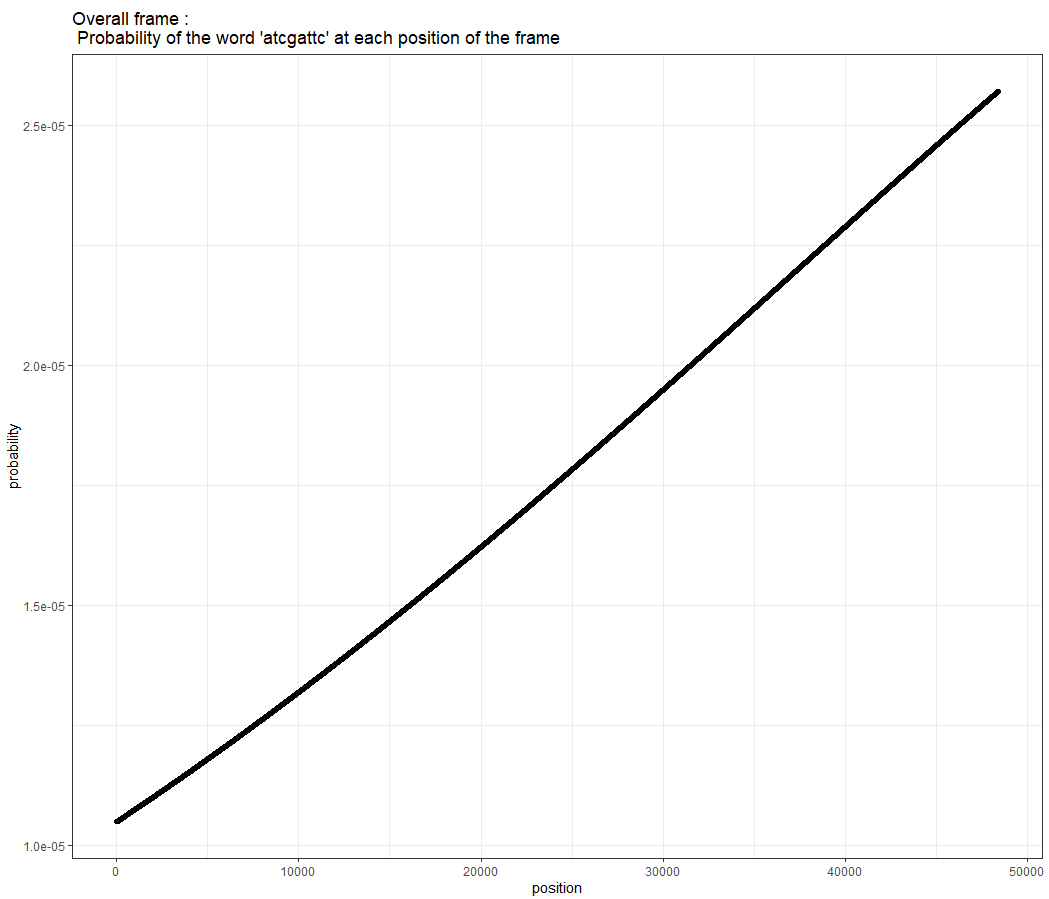
\includegraphics[width=0.6\textwidth]{wordsprobas1}
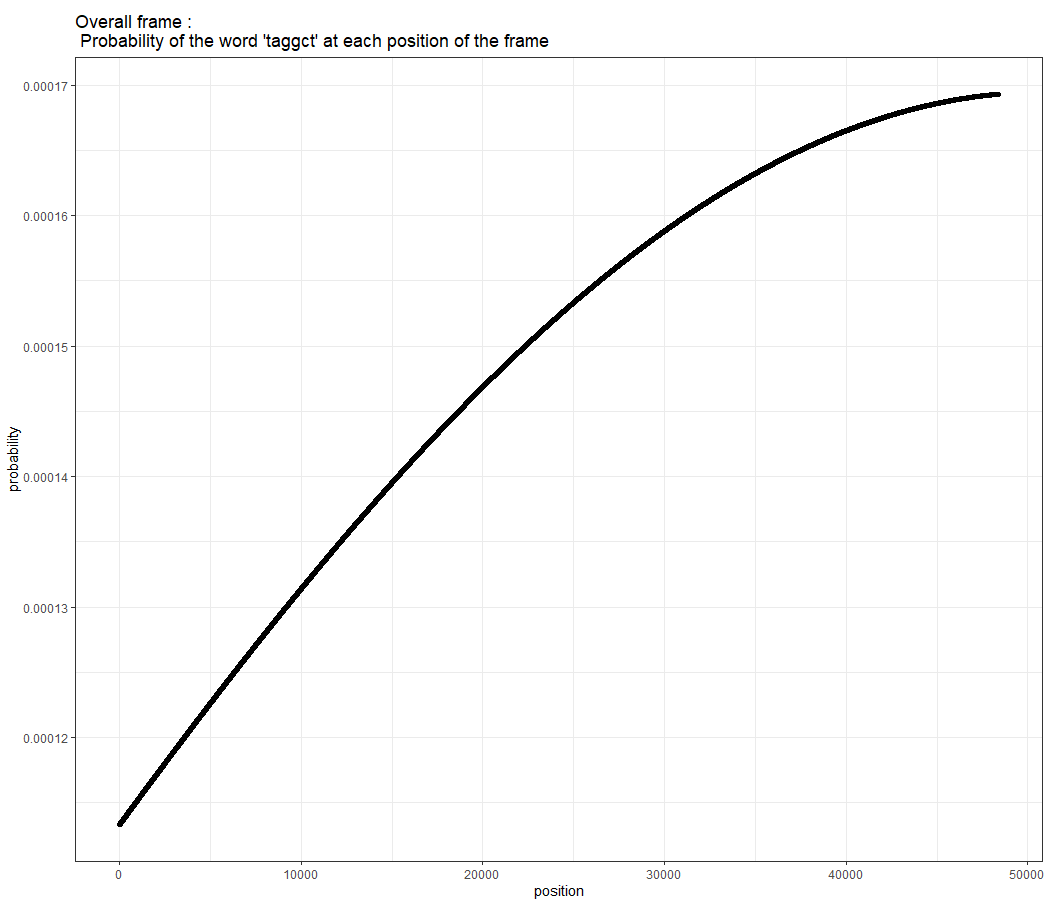
\includegraphics[width=0.6\textwidth]{wordsprobas2}
\includegraphics[width=0.6\textwidth]{wordsprobas3}
\caption{Figure plot of probabilities for each word along the sequence between <start> and <end> of {\tt pos} argument} \label{wordprobas}
\end{figure}

\clearpage

\begin{enumerate}
	\item[2.] The function \verb|length_probas| computes the probabilities of occurrence of the observed word of given size in a sequence at several positions. This function has the following {\bf arguments}:
	\end{enumerate}
%
\begin{itemize}
\item {\tt n}: Integer, the given length of the word
\item {\tt sequence}: Vector of characters representing the sequence
\item {\tt pos}: Vector of integer positions of the word along the sequence. It it is given by a {\tt start} and {\tt end} point
\item {\tt x}: An object of class {\tt dmm}
\item {\tt output\_file} A file containing the vector of probabilities
\item {\tt plot} display several figure plots of probabilities of appearance of words along the positions if TRUE
\end{itemize}
%
It returns a data frame of probability by position \\

\begin{lstlisting}
data(lambda, package = "drimmR")
dmm <- dmmsum(lambda, 1, 1, c('a','c','g','t'), init.estim = "freq")
PROB.out <- "C:\\...\\file.txt"
res <- length_probas(n=2, lambda, c(100,length(lambda)-1), dmm,
output_file=PROB.out, plot=TRUE)
\end{lstlisting}


\begin{lstlisting}
   position word        probability
1          1   gg 0.0920149143338398
2          2   gg 0.0920137134362522
3          3   gc 0.0961580205303848
4          4   cg 0.0869006631431165
5          5   gg 0.0920101107824605
6          6   gc 0.0961552204073731
7          7   cg 0.0868975633651543
8          8   ga 0.0739442789031447
9          9   ac 0.0543989570401243
10        10   cc 0.0637602384067068
\end{lstlisting}



\begin{figure}[htbp]
\centering
\includegraphics[width=0.8\textwidth]{lprobas1}
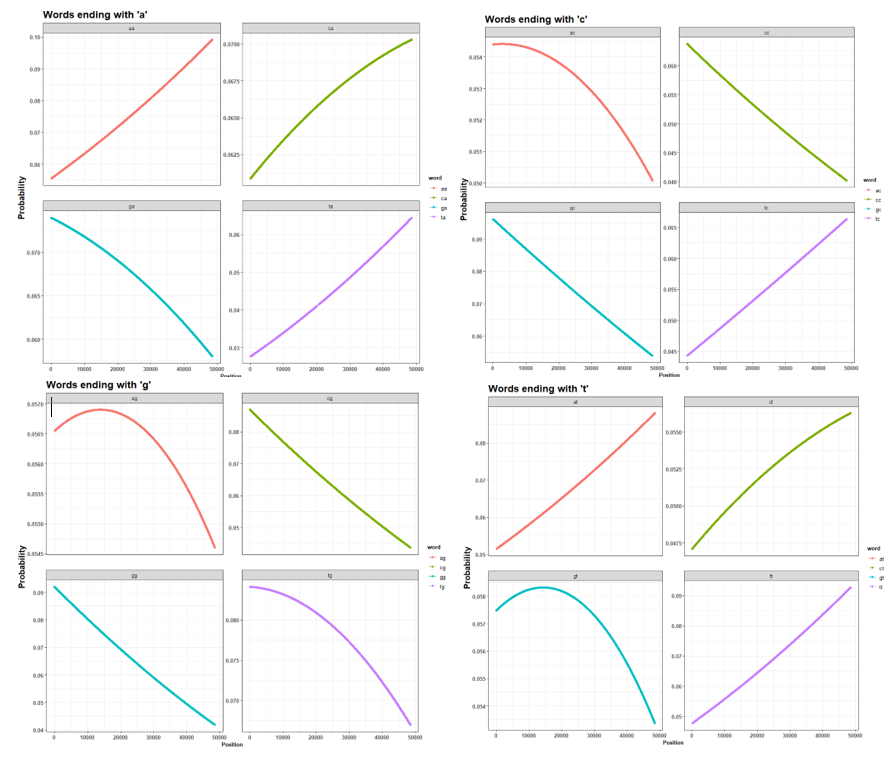
\includegraphics[width=1.03\textwidth]{lprobasv2}
\caption{Figure plot of probabilities of appearance of words of size  {\tt n} along the sequence between <start> and <end> of {\tt pos} argument} \label{wordprobas}
\end{figure}


\clearpage

\subsection{Simulation of drifting Markov models} \label{subsection_pack_simul}

The simulation of drifting Markov models is carried out by the function \verb|simulation| that has the following {\bf arguments}:
%
\begin{itemize}
\item {\tt DRIMM}: An object of class {\tt dmm}
\item \verb|output_file|: File containing the simulated sequence
\item \verb|model_size|: Integer, the size of the model
\end{itemize}

\begin{lstlisting}
data(lambda, package = "drimmR")
SIM.out <- "C:\\...\\file.txt"
dmm <- dmmsum(lambda, 1, 1, c('a','c','g','t'), init.estim = "freq")
# simulate a sequence of length 20 000 from dmm
simulate(dmm,SIM.out,20000)
\end{lstlisting}

\begin{lstlisting}
 "Write a simulated file from the model"
   [1] "t" "a" "g" "g" "g" "t" "c" "a" "t" "c" "g" "c" "c" "g" "g" "c" "g" "c"
   "c" "g" "c" "c" "a" "a" "a" "g" "g" "a" "t" "t" "c" "g" "t" "t" "t" "g" "a"
  [38] "g" "c" "c" "g" "t" "c" "t" "c" "g" "g" "g" "a" "t" "c" "a" "t" "c" "g"
  "g" "g" "g" "c" "t" "t" "c" "t" "g" "c" "t" "g" "c" "g" "t" "c" "t" "c" "c"
  [75] "g" "g" "a" "c" "g" "g" "t" "c" "t" "g" "a" "t" "t" "t" "g" "g" "c" "g"
  "g" "g" "g" "g" "a" "g" "c" "t" "g" "g" "a" "g" "g" "g" "c" "g" "g" "g" "t"
  ...
\end{lstlisting}


\clearpage

\subsection{Reliability of drifting Markov models} \label{subsection_pack_reliab}

The reliability measures are computed by means of the following functions: {\tt  A} (availability), {\tt  R} (reliability,survival function), {\tt  M} (maintainability), \verb|errorRate| (the classical failure rate, called BMP-failure rate and a more recent failure rate adapted to discrete data, called RG-failure rate). For more details on these reliability measures one can see \cite{Bar2004b,Bar2008b}. All these functions have the following {\bf arguments}:
%
\begin{itemize}
\item {\tt x}: An object of class {\tt dmm}
\item \verb|k1|: An integer, start position for the computation of the corresponding reliability measure
\item \verb|k2|: An integer, end position for the computation of the corresponding reliability measure
\item \verb|s1|: Character vector of the subspace working states (up-states) among the state space vector s.t. s1 < s
\item \verb|output_file|: File containing the estimated/computed values of the corresponding reliability measure at each position of the selected frame
\item \verb|plot|: display figure plot of the corresponding reliability measure along the positions if TRUE
\end{itemize}

The function \verb|errorRate| enables to select the type of evaluated failure rate with an additional argument :

\begin{itemize}
\item \verb|error.rate|: Default="BMP", then BMP-failure-rate is the method used to estimate the error rate. If error.rate= "RG",
then RG-failure rate is the method used to estimate the error rate.
\end{itemize}

These functions return vectors with the values of the corresponding reliability measure.

\clearpage

\subsubsection{Estimation of reliability} \label{subsection_pack_reliab}


\begin{lstlisting}
data(lambda, package = "drimmR")
dmm <- dmmsum(lambda,1,1,c("a","c","g","t"))
REL.out <- "C:\\...\\file.txt"
R(dmm,k1=1, k2=10,s1=c("a","c"),output_file = REL.out, plot=TRUE)
\end{lstlisting}


\begin{lstlisting}
     positions  reliability
 [1,]         0 1.0000000000
 [2,]         1 0.4885571729
 [3,]         2 0.2411445408
 [4,]         3 0.1188995038
 [5,]         4 0.0586239943
 [6,]         5 0.0289048794
 [7,]         6 0.0142517252
 [8,]         7 0.0070269076
 [9,]         8 0.0034646676
[10,]         9 0.0017082814
[11,]        10 0.0008422825
\end{lstlisting}


\begin{figure}[htbp]
\centering
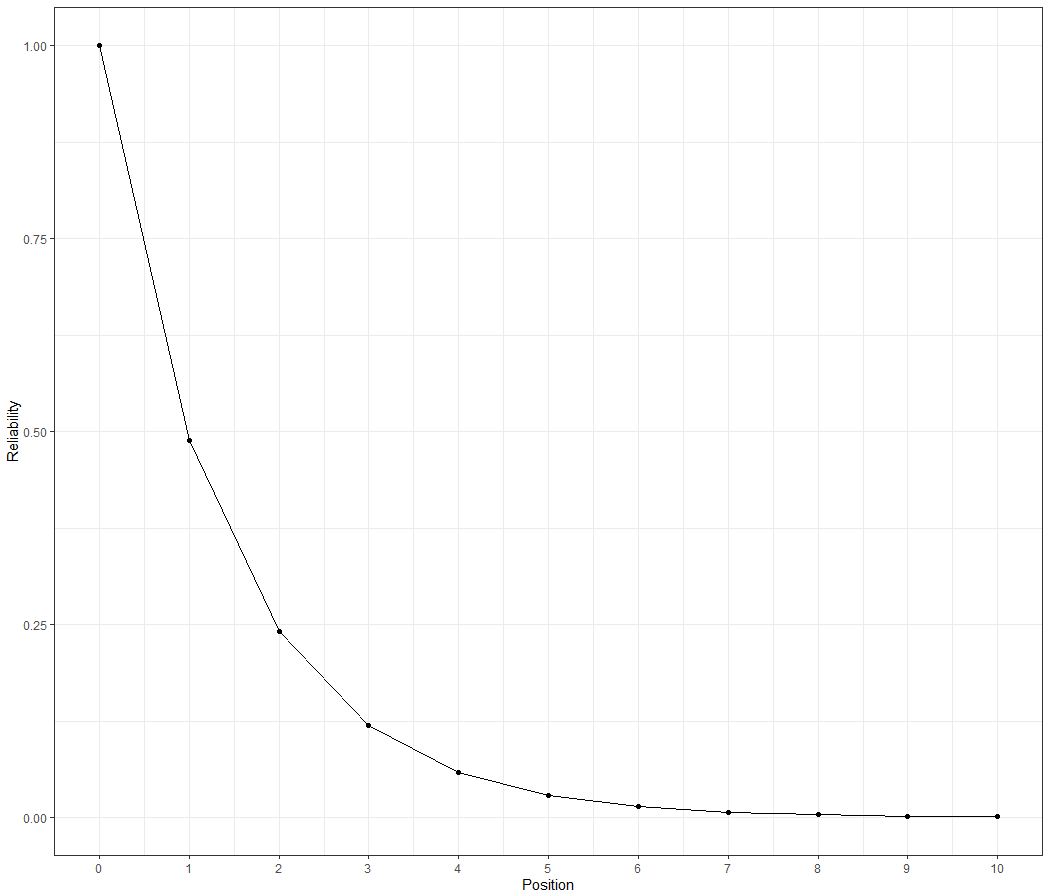
\includegraphics[width=0.7\textwidth]{rel}
\caption{Figure plot of reliability probabilities along the sequence between {\tt k1} and {\tt k2} position arguments for the working states subspace  {\tt s1} }
\end{figure}

\clearpage

\subsubsection{Estimation of availability} \label{subsection_pack_avail}


\begin{lstlisting}
 data(lambda, package = "drimmR")
dmm <- dmmsum(lambda,1,1,c("a","c","g","t"))
AVA.out <- "C:\\...\\file.txt"
A(dmm,k1=1, k2=10,s1=c("a","c"),output_file = AVA.out, plot=TRUE)
\end{lstlisting}

\begin{lstlisting}
    positions availability
 [1,]         0    0.4885572
 [2,]         1    0.4690808
 [3,]         2    0.4761674
 [4,]         3    0.4766474
 [5,]         4    0.4766457
 [6,]         5    0.4766422
 [7,]         6    0.4766424
 [8,]         7    0.4766428
 [9,]         8    0.4766432
[10,]         9    0.4766436
[11,]        10    0.4766440
\end{lstlisting}

\begin{figure}[htbp]
\centering
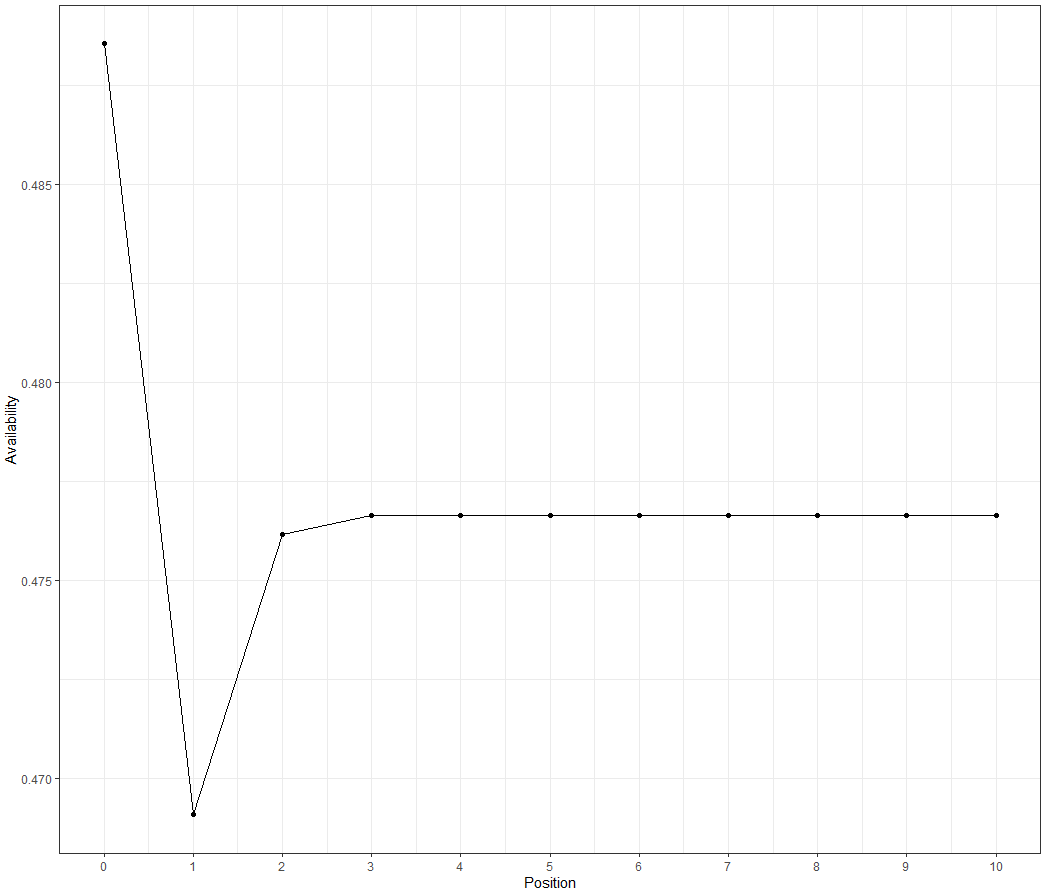
\includegraphics[width=0.7\textwidth]{ava}
\caption{Figure plot of availability probabilities along the sequence between {\tt k1} and {\tt k2} position arguments for the working states subspace  {\tt s1} }
\end{figure}

\clearpage


\subsubsection{Estimation of maintainability} \label{subsection_pack_maintain}


\begin{lstlisting}
 data(lambda, package = "drimmR")
dmm <- dmmsum(lambda,1,1,c("a","c","g","t"))
MAIN.out <- "C:\\...\\file.txt"
M(dmm,k1=1, k2=10,s1=c("a","c"),output_file = MAIN.out, plot=TRUE)
\end{lstlisting}

\begin{lstlisting}
      positions maintainability
 [1,]         0       0.0000000
 [2,]         1       0.4885572
 [3,]         2       0.7164935
 [4,]         3       0.8485148
 [5,]         4       0.9189865
 [6,]         5       0.9566753
 [7,]         6       0.9768307
 [8,]         7       0.9876094
 [9,]         8       0.9933737
[10,]         9       0.9964564
[11,]        10       0.9981049
\end{lstlisting}

\begin{figure}[htbp]
\centering
\includegraphics[width=0.7\textwidth]{main}
\caption{Figure plot of availability probabilities along the sequence between {\tt k1} and {\tt k2} position arguments for the working states subspace  {\tt s1} }
\end{figure}



\clearpage

\subsubsection{Estimation of failure rates} \label{subsection_pack_reliab}


\begin{lstlisting}
 data(lambda, package = "drimmR")
dmm <- dmmsum(lambda,1,1,c("a","c","g","t"))
ER.out <- "C:\\...\\file.txt"
errorRate(mod,1,10,c("a","c"), error.rate="BMP", output_file=ER.out, plot=TRUE)
\end{lstlisting}

\begin{lstlisting}
      positions       BMP
 [1,]         0 0.0000000
 [2,]         1 0.5114428
 [3,]         2 0.5064149
 [4,]         3 0.5069368
 [5,]         4 0.5069450
 [6,]         5 0.5069446
 [7,]         6 0.5069440
 [8,]         7 0.5069434
 [9,]         8 0.5069428
[10,]         9 0.5069422
[11,]        10 0.5069416
\end{lstlisting}


\begin{figure}[htbp]
\centering
\includegraphics[width=0.7\textwidth]{er}
\caption{Figure plot of BMP-failure rates along the sequence between {\tt k1} and {\tt k2} position arguments for the working states subspace  {\tt s1} }
\end{figure}

\clearpage

\section{Concluding remarks} \label{concluding}

To conclude, in this paper we have presented {\tt drimmR}, an {\tt R} package for  simulation, estimation and reliability and survival analysis of drifting Markov models. These are versatile stochastic models of Markov type capable of taking into account a time non-homogeneity of a known, controlled shape. For this reason these models can represent interesting modeling alternatives to classical models (like Markov models, semi-Markov models, etc.) and can be useful for researchers, practitioners and engineers in various fields.

The package addresses several items important from practical point of view, when carrying out the estimation: we consider one or several samples, the sample paths can be complete or not, can come from models of the same length or of different lengths.

The fields of application of the DMMs can be numerous; we only want to point out three of them.

\begin{itemize}
\item  \emph{Survival analysis} and \emph{reliability theory}: note that important indicators like reliability or survival function, availability, maintainability and failure rates are computed in our package;
\item  \emph{Bioinformatics}: note that important quantities for OMICS data in general,  DNA analysis in particular, are computed by the proposed package. Thus we have the computation of the  probabilities and expectations of  appearance of a given word along the sequence.

\end{itemize}


\clearpage

\bibliography{drimmr}

\printbibliography


\begin{figure}[htbp]
\centering
\includegraphics[width=0.7\textwidth]{fig}
\caption{Flowchart of the \tt{drimmR} package. } \label{fig}
\end{figure}


\end{document}
